\documentclass[12pt]{article}

\usepackage{tikz}

\begin{document}
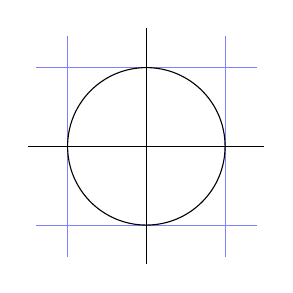
\begin{tikzpicture}
  [our grid/.style = {help lines, color=#1!50},
   our grid/.default=blue]
  
  \draw[our grid] (-1.4, -1.4) grid (1.4, 1.4);
  % left corner -- right corner of the grid
  \draw (-1.5, 0) -- (1.5, 0);
  \draw (0, -1.5) -- (0, 1.5);
  \draw (0,0) circle (1cm);
\end{tikzpicture}

\begin{tikzpicture}[ultra thick]
  \draw (0,0) -- (0,1);
  \begin{scope}[thin]
    \draw (1,0) -- (1,1);
    \draw (2,0) -- (2,1);
  \end{scope}
  \draw (3,0) -- (3,1);
\end{tikzpicture}

\end{document}